\chapter{Material und Methoden}
\section{Chemikalien}
Die in dieser Arbeit verwendeten Chemikalien waren von analytischem Reinheitsgrad und wurden, soweit im Text nicht anders angegeben, von folgenden Herstellern bezogen:\\
%\vspace{5mm}\\
\begin{tabular}[H]{p{.25\textwidth}l}
AppliChem&AppliChem GmbH, Darmstadt\\
Fluka&Sigma-Aldrich Chemie GmbH, Taufkirchen\\
Merck&Merck KGaA, Darmstadt\\
Riedel-deHa\"en&Sigma-Aldrich Chemie GmbH, Taufkirchen\\
Roth&Carl Roth GmbH \& Co. KG, Karlsruhe\\
Serva&Serva Electrophoresis GmbH, Heidelberg\\
SIGMA&Sigma-Aldrich Chemie GmbH, Steinheim\\ 
\end{tabular}
\subsection{Antibiotika und Naturstoffe}
Für die in dieser Arbeit verwendeten Antibiotika und Naturstoffe wurden Stammlösungen angesetzt, welche bis zu ihrer Verwendung bei -20\celcius\ gelagert wurden. Die Konzentration der Stammlösungen sowie das jeweilige Lösungsmittel sind in \Fref{tab:AB} aufgelistet.\\
%\begin{table}[H]
\captionof{table}[Verwendete Antibiotika und Naturstoffe]{Liste der verwendeten Antibiotika und Naturstoffe}
\label{tab:AB}
\begin{tabular}
{
p{.2\textwidth}
S[table-format=1.0,table-comparator=true,table-space-text-post={**********************}]
p{.45\textwidth}
}
\toprule
\multicolumn{1}{l}{Substanz}&\multicolumn{1}{l}{Konzentration} & \multicolumn{1}{l}{Hersteller}\\ 
\midrule
Acetosyringon & 200\,\si{mM}~in~ \acs{EtOH}& Carl Roth GmbH, Karlsruhe \\ 
Ampicilin & 100\,\si{mg\per ml}~ in~ \acs{\reinstwasser} & AppliChem GmbH, Darmstadt \\ 
Kanamycin & 50\,\si{mg\per ml} ~in~\acs{\reinstwasser} & Duchefa B.V, Haarlem, NL  \\ 
Spectinomycin & 100\,\si{mg\per ml}~ in~ \acs{\reinstwasser} & Sigma-Aldrich GmbH, Steinheim \\ 
Rifampicin & 50\,\si{mg\per ml} ~in~ DMSO & Duchefa B.V, Haarlem, NL \\ 
\bottomrule
\end{tabular}
%\end{table}
\vspace{12pt}\\
Soweit im Text nicht anders angegeben, wurden Ampicilin und Spectinomycin in einer Endkonzentration von 100\,$\mu$g/ml, Kanamycin und Rifampicin in einer Endkonzentration von 50\,$\mu$g/ml eingesetzt. Acetosyringon wurde in einer Endkonzentration von 200\,$\mu$M verwendet. 
\newpage
%\section{Nährmedien, Puffer und Lösungen}
\subsection{Nährmedien}
%\vspace{12pt}
%Alle Nährmedien wurden mit \acs {\vewasser} angesetzt und anschließend für 20\,min bei 120\celcius~autoklaviert. Für die Herstellung von festen Nährmedien wurden die Medien vor dem Autoklavieren mit 1,7\si{\%}(w/v) Agar ergänzt. 
%\begin{table}[H]
\begin{longtable}{
p{.3\textwidth}
p{.3\textwidth}
S[table-format=1.3,table-comparator=true,table-space-text-post={*****}]
p{.3\textwidth}
}
\acs{LB}-Medium & Bacto-Trypton & 1\%(w/v) &  \\ 
 & Hefeextrakt & 0,5\si{\%}(w/v) &  \\ 
 & NaCl & 1\si{\%}(w/v) &  \\ 
 & pH & 7,0 &  \\ 
 &  &  &  \\ 
\acs{TB}-Medium & Bacto-Trypton & 1\si{\%}(w/v) &  \\ 
 & Hefeextrakt & 2,4\si{\%}(w/v) &  \\ 
 & Glycerin & 0,4\si{\%}(v/v) &  \\ 
 \begin{tabular}{
p{.285\textwidth}
p{.5\textwidth}
%p{1cm}
S[table-format=1.3,table-comparator=true,table-space-text-post={*****}]
p{.3\textwidth}}
&Das Medium wurde autoklaviert und  abgekühlt. Anschließend wurden 10\,\si{\%}\ (v/v) KPO$_4$-Puffer zugegeben. Die weitere Lagerung erfolgte bei Raumtemperatur.
\end{tabular}\\
&&&\\ 
SOB-Medium& Bacto-Trypton& 2\si{\%}(w/v) &  \\ 
 & Hefeextrakt & 0,5\si{\%}(w/v) &  \\ 
 &KCL& 2,5\si{mM}&\\
 & NaCl & 10\si{mM} &  \\
   \begin{tabular}{
p{.285\textwidth}
p{.5\textwidth}
%p{1cm}
S[table-format=1.3,table-comparator=true,table-space-text-post={*****}]
p{.3\textwidth}}
&Das Medium wurde autoklaviert und bei Raumtemperatur gelagert. Direkt vor der Verwendung, wurde MgSO$_4$ zu einer Endkonzentration von 10\,\si{mM}  zugegeben.&&\\
\end{tabular}\\
&&&\\
\acs{SOC}-Medium & Bacto-Trypton & 2\si{\%}(w/v) &  \\ 
 & Hefeextrakt & 0,5\si{\%}(w/v) &  \\ 
 & NaCl & 10\si{mM} &  \\ 
 & KCl & 2,5\si{mM} &  \\ 
 & MgCl$_2$ & 10\si{mM} &  \\ 
 & MgSO$_4$ & 10\si{mM} &  \\ 
   \begin{tabular}{
p{.285\textwidth}
p{.5\textwidth}
%p{1cm}
S[table-format=1.3,table-comparator=true,table-space-text-post={*****}]
p{.3\textwidth}}
&Das Medium wurde autoklaviert und  abgekühlt. Anschließend wurde Glukose zu einer Endkonzentration von 20\,\si{mM}\ zugegeben. Die weitere Lagerung erfolgte bei Raumtemperatur.
\end{tabular}\\
&&&\\ 
\newpage 
 YEB-Medium & Pepton & 5\si{\%}(w/v) &  \\ 
 & Hefeextrakt & 1\si{\%}(w/v) &  \\ 
 & Fleischextrakt & 5\si{\%}(w/v) &  \\ 
 & Saccharose & 5\si{\%}(w/v) &  \\ 
 & MgSO$_4$ & 2\si{mM} &  \\ 
 & pH & 7,2 &  \\ 
\end{longtable}
\addtocounter{table}{-1}
\subsection{Puffer und Lösungen}
    \begin{longtable}{ 
 p{.3\textwidth}
p{.3\textwidth}
%p{1cm}
S[table-format=1.3,table-comparator=true,table-space-text-post={*****}]
p{.3\textwidth}}
Anilinblau& Anilinblau& 0,05\si{\%}\ (w/v)& \\
&Glyzerin& 50\si{\%}\ (v/v)&\\
&Milchsäure&25 \si{\%}\ (v/v)&\\
&&&\\
EDTA&EDTA&0,5\si{M}&\\
&pH (NaOH)& 8,0&\\
\begin{tabular}{
p{.29\textwidth}
p{.5\textwidth}
%p{1cm}
S[table-format=1.3,table-comparator=true,table-space-text-post={*****}]
p{.3\textwidth}}
&Die Lösung wurde autoklaviert und bei Raumtemperatur gelagert.&&\\
\end{tabular}\\
&&&\\
\acs{GUS}-Färbepuffer & NaPO$_4$-Puffer (1\si{M}) & 50\si{mM} &   \\ 
& \acs{EDTA} & 10\si{mM} &  \\ 
& K$_3$Fe(CN)$_6$ & 0,5\si{mM} &  \\ 
& K$_4$Fe(CN)$_6$ & 0,5\si{mM} &  \\ 
& Triton X-100 & 0,1\si{\%}\ (v/v) &  \\ 
& \acs{X-Gluc} & 2\si{mM} &  \\ 
\begin{tabular}{
p{.29\textwidth}
p{.5\textwidth}
%p{1cm}
S[table-format=1.3,table-comparator=true,table-space-text-post={*****}]
p{.3\textwidth}}
&Der Puffer ist nur eingeschränkt lagerfähig und wurde daher unmittelbar vor Gebrauch angesetzt.&&\\
\end{tabular}\\
&  &  &  \\ 
\acs{HEPES} & \acs{HEPES} & 1\si{mM} &  \\ 
 & pH (NaOH) & 7,0 &  \\ 
\begin{tabular}{
p{.29\textwidth}
p{.5\textwidth}
%p{1cm}
S[table-format=1.3,table-comparator=true,table-space-text-post={*****}]
p{.3\textwidth}}
&Der Puffer wurde durch einen Filter mit 0,2\,$\mu$m Porenweite sterilfiltriert und bei 4\celcius\ gelagert.&&\\
\end{tabular}\\
&&&\\
\acs{HEPES}-Puffer 1 & \acs{HEPES} & 1\si{\%}\ (v/v) &  \\ 
\begin{tabular}{
p{.29\textwidth}
p{.5\textwidth}
%p{1cm}
S[table-format=1.3,table-comparator=true,table-space-text-post={*****}]
p{.3\textwidth}}
&Der Puffer wurde durch einen Filter mit 0,2\,$\mu$m Porenweite sterilfiltriert und bei 4\celcius\ gelagert.&&\\
\end{tabular}\\
&  &  &  \\ 
\acs{HEPES}-Puffer 2 & \acs{HEPES} & 1\si{\%}\ (v/v)&  \\ 
& Glyzerin & 10\si{\%}\ (v/v) &  \\ 
\begin{tabular}{
p{.29\textwidth}
p{.5\textwidth}
%p{1cm}
S[table-format=1.3,table-comparator=true,table-space-text-post={*****}]
p{.3\textwidth}}
&Der Puffer wurde durch einen Filter mit 0,2\,$\mu$m Porenweite sterilfiltriert und bei 4\celcius\ gelagert.&&\\
\end{tabular}\\
&  &  &  \\ 
Infiltrationspuffer & \acs{MES} & 10\si{mM} &  \\ 
& MgCl$_2$ & 10\si{mM} &  \\ 
& Acetosyringon  & 200\si{$\mu$M} &  \\ 
\begin{tabular}{
p{.29\textwidth}
p{.5\textwidth}
%p{1cm}
S[table-format=1.3,table-comparator=true,table-space-text-post={*****}]
p{.3\textwidth}}
&Der Puffer ist nur eingeschränkt lagerfähig und wurde daher unmittelbar vor Gebrauch angesetzt.&&\\
\end{tabular}\\
&  &  &  \\ 
KPO$_4$-Puffer & KH$_2$PO$_4$ & 0,17\si{M} &  \\ 
& K$_2$HPO$_4$ & 0,72\si{M} &  \\ 
\begin{tabular}{
p{.29\textwidth}
p{.5\textwidth}
%p{1cm}
S[table-format=1.3,table-comparator=true,table-space-text-post={*****}]
p{.3\textwidth}}
&Der Puffer wurde autoklaviert und bei Raumtemperatur gelagert.&&\\
\end{tabular}\\
&  &  &  \\ 
\acs{MES}&\acs{MES}&500\si{mM}&\\
&pH (NaOH) & 5,6&\\
\begin{tabular}{
p{.29\textwidth}
p{.5\textwidth}
%p{1cm}
S[table-format=1.3,table-comparator=true,table-space-text-post={*****}]
p{.3\textwidth}}
&Der Puffer wurde durch einen Filter mit 0,2\,$\mu$m Porenweite sterilfiltriert und bei 4\celcius\ gelagert.&&\\
\end{tabular}\\
&&&\\
%\acs{MOPS} (10fach) & \acs{MOPS} & 400\si{mM} &  \\ 
%& Natriumacetat & 100\si{mM} &  \\ 
%& \acs{EDTA} & 10\si{mM} &  \\ 
%&  &  &  \\ 
Na$_2$HPO$_4$&Na$_2$HPO$_4$& 1\si{M}&\\
\begin{tabular}{
p{.29\textwidth}
p{.5\textwidth}
%p{1cm}
S[table-format=1.3,table-comparator=true,table-space-text-post={*****}]
p{.3\textwidth}}
&Die Lösung wurde autoklaviert und bei Raumtemperatur gelagert.&&\\
\end{tabular}\\
&&&\\
NaH$_2$PO$_4$ &NaH$_2$PO$_4$ & 1\si{M}&\\
\begin{tabular}{
p{.29\textwidth}
p{.5\textwidth}
%p{1cm}
S[table-format=1.3,table-comparator=true,table-space-text-post={*****}]
p{.3\textwidth}}
&Die Lösung wurde autoklaviert und bei Raumtemperatur gelagert.&&\\
\end{tabular}\\
&&&\\
NaPO$_4$-Puffer & Na$_2$HPO$_4$ (\si{1M}) & 72\si{\%}\ (v/v) &  \\ 
  &NaH$_2$PO$_4$ (\si{1M}) & 28\si{\%}\ (v/v) &  \\ 
 & pH & 7,2 &  \\ 
\begin{tabular}{
p{.29\textwidth}
p{.5\textwidth}
%p{1cm}
S[table-format=1.3,table-comparator=true,table-space-text-post={*****}]
p{.3\textwidth}}
&Der Puffer wurde autoklaviert und bei Raumtemperatur gelagert.&&\\
\end{tabular}\\
&&&\\
\newpage
PIPES & Pipes-Na$_2$&500\,mM&\\
						&	pH&6,7&\\
\begin{tabular}{
p{.29\textwidth}
p{.5\textwidth}
%p{1cm}
S[table-format=1.3,table-comparator=true,table-space-text-post={*****}]
p{.3\textwidth}}
&Der Puffer wurde durch einen Filter mit 0,2\,$\mu$m Porenweite sterilfiltriert und bei 4\celcius\ gelagert.&&\\
\end{tabular}\\
&&&\\
\acs{TAE} (50fach) & \acs{TRIS} & 2\si{M} &  \\ 
 & Eisessig & 5,7\si{\%}\ (v/v) &  \\ 
 & \acs{EDTA} (0,5M) & 50\si{mM} &  \\ 
 & pH  & 8,0 &  \\ 
\begin{tabular}{
p{.29\textwidth}
p{.5\textwidth}
%p{1cm}
S[table-format=1.3,table-comparator=true,table-space-text-post={*****}]
p{.3\textwidth}}
&Zur Verwendung wurde der Puffer 1:50 mit \vewasser\ verdünnt.&&\\
\end{tabular}\\
&  &  &  \\ 
TB-Puffer& CaCl$_2$ & 15\,mM&\\
	&KCL&250\,mM&\\
	&PIPES&10\,mM&\\
	&\multicolumn{3}{l}{pH mit 1\,M KOH auf 6,7 einstellen}\\
&MnCl$_2$&55\,mM&\\
\begin{tabular}{
p{.29\textwidth}
p{.5\textwidth}
%p{1cm}
S[table-format=1.3,table-comparator=true,table-space-text-post={*****}]
p{.3\textwidth}}
&Der Puffer wurde durch einen Filter mit 0,2\,$\mu$m Porenweite sterilfiltriert und bei 4\celcius\ gelagert.&&\\
\end{tabular}\\
&&&\\
\acs{TBE} (5fach) & \acs{TRIS} & 445\si{mM} &  \\ 
 & Borsäure & 445\si{mM} &  \\ 
 & \acs{EDTA}  & 10\si{mM} &  \\ 
\begin{tabular}{
p{.29\textwidth}
p{.5\textwidth}
%p{1cm}
S[table-format=1.3,table-comparator=true,table-space-text-post={*****}]
p{.3\textwidth}}
&Zur Verwendung wurde der Puffer 1:10 mit \vewasser\ verdünnt.&&\\
\end{tabular}\\
&  &  &  \\ 
\end{longtable}
\addtocounter{table}{-1}
\newpage
\section{Verbrauchsmaterialien}
\subsection{Kits}
Die in dieser Arbeit verwendeten Enzyme und Kits sowie die jeweiligen Hersteller sind in \Fref{tab:Enzyme} und \Fref{tab:Kits} aufgelistet.\\
\captionof{table}[Verwendeten Kits]{Liste der verwendeten Kits}
\label{tab:Kits}
\begin{tabular}{l
l
l
}
\toprule
Bezeichnung & Verwendung&Hersteller \\ 
\midrule
peqGold Cycle Pure Kit & PCR-Aufreinigung  & Peqlab GmbH, Erlangen\\  
peqGold Gel Extraction Kit & DNA Gelextraktion & Peqlab GmbH, Erlangen \\
peqGold Plasmid Mini Kit & Plasmidisolation & Peqlab GmbH, Erlangen\\
Plant RNA Isolation Kit & RNA Isolation & Agilent GmbH, Böblingen\\ 
Qubit RNA BR Assay Kit & RNA-Quantifizierung & Life Technologies,\\
&&Carlsbad, USA \\ 
Qubit DNA BR Assay Kit & DNA-Quantifizierung & Life Technologies,\\
& & Carlsbad, USA \\ 
Sensifast Probe no-ROX Kit & Real Time PCR & Bioline GmbH,\\ 
&&Luckenwalde\\
Sensifast Sybr no-ROX Kit & Real-Time PCR & Bioline GmbH, \\
&&Luckenwalde\\
Tetro cDNA Synthese Kit & cDNA-Synthese & Bioline GmbH, \\
&&Luckenwalde\\
\bottomrule
\end{tabular}
\vspace{12pt}
\subsection{Enzyme}
\captionof{table}[Verwendete Enzyme]{Liste der verwendeten Enzyme}
\label{tab:Enzyme}
\begin{tabular}{
l
l
l
}
\toprule
Bezeichnung & Enzym & Hersteller\\
\midrule
DNA-free &RNAse-freie DNAse& Life Technologies,\\
&&Carlsbad, CA, USA\\
FastAP & Alkalische Phosphatase & Fisher Scientific GmbH, Schwerte\\
FastDigest \BamHI & Restriktionsendonuklease & Fisher Scientific GmbH, Schwerte\\
FastDigest \EcoRI & Restriktionsendonuklease & Fisher Scientific GmbH, Schwerte\\
FastDigest \ClaI & Restriktionsendonuklease & Fisher Scientific GmbH, Schwerte\\
FastDigest \KpnI & Restriktionsendonuklease & Fisher Scientific GmbH, Schwerte\\
FastDigest \XbaI & Restriktionsendonuklease & Fisher Scientific GmbH, Schwerte\\
FastDigest \XhoI & Restriktionsendonuklease & Fisher Scientific GmbH, Schwerte\\
MightyMix & T4 DNA Ligase & Takara Bio Europe S.A.S,\\
 &&Saint-Germain-en-Laye, FR\\
Phusion &  DNA Polymerase & Fisher Scientific GmbH, Schwerte\\
\textit{Taq} Polymerase &  DNA Polymerase & Fisher Scientific GmbH, Schwerte\\
\bottomrule
\end{tabular}
%\vspace{12pt}\\
\subsection{Oligonukleotide}
Die Synthese von Oligonukleotiden für konventionelle \acs{PCR}-Anwendungen erfolgte bei der Biomers.net~GmbH, Ulm.
Oligonukleotide und \TaqMan\,-Sonden für real-time \acs{PCR}-Anwendungen waren  \acs{HPLC}-gereinigt und wurden von der Apara~Bioscience~GmbH, Denzlingen bezogen.
\subsection{Klonierungsprimer}
Die in dieser Arbeit verwendeten Klonierungsprimer sind in \Fref{tab:Kloprimer} aufgelistet. Diese Primer wurden mit 5'-Überhängen entworfen,  um DNA-Fragmente mit Restriktionsschnittstellen zu amplifizieren. Die so erzeugten PCR-Produkten konnten nach einem Restriktionsverdau in Plasmidvektoren ligiert werden. Zusätzlich zu den palindromischen Erkennungssequenzen wurden jeweils drei Schutzbasen angehängt.\\
\captionof{table}[Klonierungsprimer]{Liste der verwendeten Klonierungsprimer}
\label{tab:Kloprimer}
\setlength{\LTpre}{0pt}
\setlength{\LTpost}{0pt}
\small
\begin{longtable}{
p{.13\textwidth}
p{.57\textwidth}
p{.075\textwidth}
p{.12\textwidth}
}
\toprule
Bezeichnung & Überhang - Sequenz (5'$\rightarrow$3') & Tm\,(\celcius) & Schnittstelle\\
\midrule
\endhead
00415fw & TGAGGATCC-CACCTGCTCGTCCTAC & 70 & \BamHI \\ 
00415rv & TGAGGATCC-TGCTTACGCCGTTATATTGCC & 71 & \BamHI \\ 
01251fw & TGGGATCC-AAACTGTTGGCTTTTGATCCAT & 70 & \BamHI \\ 
01251rv & TGAGGATCC-TATCTGCCCCCTCATTTACACT & 71 & \BamHI \\ 
01371fw & CTGGGATCC-TGGCTTTTCTATCAGCAAGTGA & 71 & \BamHI \\ 
01371rv & TGAGGATCC-TCCCAGATCTAGTCCACCATCT & 72 & \BamHI \\ 
01750fw & TGAGGATCC-GCCTTCGCCAAGGAGACTTA & 72 & \BamHI \\ 
01750rv & TGAGGATCC-GGCAGTTGGCACATCAGTTG & 73 & \BamHI \\ 
04224fw & TGAGGATCC-CAGTCGTTGCCACCAAGTGT & 72 & \BamHI \\ 
04224rv & TGAGGATCC-CACGGCGACACCAATCATTA & 74 & \BamHI \\ 
04224\XhoI & CTACTCGAG-TTGCCACCAAGTGTACG & 68 & \XhoI \\ 
04224\KpnI & CTAGGTACC-TAGAGCACGGCGACACC & 71 & \KpnI \\ 
04224\XbaI & CTATCTAGAT-TGCCACCAAGTGTACG & 64 & \XbaI \\ 
04224\ClaI & CTAATCGAT-TAGAGCACGGCGACACC & 69 & \ClaI \\ 
05320fw & TGAGGATCC-GACTAGTGAAATATACCCTC & 66 & \BamHI \\ 
05320rv & TGAGGATCC-TCGCGTCTGTAAGCATCACT & 72 & \BamHI \\ 
06673fw & TGAGGATCC-CCTGGTTCCTTTGAACCACC & 73 & \BamHI \\ 
06673rv & TGAGGATCC-GATTTGATGTATTGATGTCTCTG & 67 & \BamHI \\ 
1976\XhoI & CTACTCGAG-GGTGCTAACTCTTC & 67 &\XhoI \\ 
1976\KpnI & CTAGGTACC-AGCCACAGTGACAATC & 66 & \KpnI \\ 
1976\XbaI & CTATCTAGA-GGTGCTAACACCTCTTC & 63 & \XbaI \\ 
1976\ClaI & CTAATCGAT-AGCCACAGTGACAATC & 63 & \ClaI \\ 
2356fw & TGAGGATCC-GGTGGGATGGGAACAGGTCGTAG & 76 & \BamHI \\ 
2356rv & TGAGGATCC-TGGTCTTGCAGTGGGAGTGATTC & 74 & \BamHI \\ 
2683\XhoI & CTACTCGAG-GTTGCTCAGTGAATAAGTC & 66 & \XhoI \\ 
2683\KpnI & CTAGGTACC-ATATGATACGAGAGGCTGTAG & 66 & \KpnI \\ 
2683\XbaI & CTATCTAGA-GTTGCTCAGTGAATAAGTC & 62 & \XbaI \\ 
2683\ClaI & CTAATCGAT-ATATGATACGAGAGGCTGTAG & 63 & \ClaI \\ 
3015fw & TGAGGATCC-GAGTTTGTAGACGGTCTGTCTGC & 73 & \BamHI \\ 
3015rv & TGAGGATCC-GAATAGAGCTTCCAGAGTCATCTG & 71 & \BamHI \\ 
462\XhoI & CTACTCGAG-GCAAAGGCTTGTATTAACG & 67 & \XhoI \\ 
462\KpnI & CTAGGTACC-GGCTCTAATTGTTTGTCAG & 66 & \KpnI \\ 
462\XbaI & CTATCTAGA-GCAAAGGCTTGTATTAACG & 63 & \XbaI \\ 
462\ClaI & CTAATCGAT-GGCTCTAATTGTTTGTCAG & 64 & \ClaI \\ 
PDS\XhoI & CTACTCGAG-AAAGAACAGCGCCTTCC & 68 & \XhoI \\ 
PDS\KpnI & CTAGGTACC-GCCCAAACCAGTCAATG & 69 & \KpnI \\ 
PDS\XbaI & CTATCTAGA-AAAGAACAGCGCCTTCC & 65 & \XbaI \\ 
PDS\ClaI & CTAATCGAT-GCCCAAACCAGTCAATG & 66 & \ClaI \\ 
iGUS\BamHI & CTAGGATCC-TCATTGTTTGCCTCCCTGCTGCGGT & 76 & \BamHI \\ 
iGUS\EcoRI & CTAGAATTC-ATGGTACGTCCTGTAGAAACCCCAA & 70 & \EcoRI \\ 
\bottomrule
\end{longtable}
\addtocounter{table}{-1}
\normalsize
\subsection{Primer und Sonden für real-time PCR-Anwendungen}
Die in \Fref{tab:realtimePrimer} aufgelisteten Primer und Sonden wurden zur Genexpressionsanalyse eingesetzt. Die Amplifikationseffizienz (E) der einzelnen Primerpaare wurde über Standardkurven bestimmt (Siehe MM Standardkurven, Siehe Anhang Stdcrv). Die verwendete \TaqMan -Sonde war mit dem Fluorophor \acs{FAM} und dem Quencher \acs{TAMRA} gelabelt.\\ 
\captionof{table}[Primer und Sonden für real-time PCR-Anwendungen]{Liste der verwendeten Primer und Sonden für real-time PCR Anwendungen}
\label{tab:realtimePrimer}
\setlength{\LTpre}{0pt}
\setlength{\LTpost}{0pt}
\small
\begin{longtable}{
L{.175\textwidth}
p{.55\textwidth}
p{.085\textwidth}
p{.055\textwidth}
}
\toprule
Bezeichnung & Sequenz 5' $\rightarrow$ 3' & Tm\,(\celcius)&E\,(\%) \\ 
\midrule
\endhead 
ActinDis1f  & ACAGTTTCACCACAACCGCC & 65 &\\ 
ActinDis1r  & TGACCGTCGGGAAGTTCG & 63 &\\ 
AtubDis1f  & CTGCGAACAACTATGCTCGTC & 63& \\ 
AtubDis1r & CACGAAGAAGCCTTGGAGTCC & 64 &\\ 
CytB1f  & TCAAGACGCATCCAAATTCTAGGTC & 64& \\ 
CytB1r  & GTGTTACACCCGTGATAATCTGAATGAT & 65& \\ 
Elf1a1f  & GTGAGCGTGGTATCACCATC & 62& \\ 
Elf1a1r  & CAGAATGGCGCAATCAGC & 61& \\ 
Elf1a2f  & GGAAATGGATACGCTCCTGTC & 62& \\ 
Elf1a2r  & CTTAACTAAGGCGGCGTCTC & 62 &\\ 
GAPDH1f  & GGTATGGCTTTCCGAGTTCCA & 64& \\ 
GAPDH1r  & TCAGTTGATACCAAATCATCCTCAG & 62 &\\ 
Gmcons4fw  & GATCAGCAATTATGCACAACG & 60 &\\ 
Gmcons4rv  & CCGCCACCATTCAGATTATGT & 62 &\\ 
Gmcons6fw  & AGATAGGGAAATGGTGCAGGT & 63 &\\ 
Gmcons6rv  & CTAATGGCAATTGCAGCTCTC & 61 &\\ 
Gmcons7fw  & ATGAATGACGGTTCCCATGTA & 61 &\\ 
Gmcons7rv  & GGCATTAAGGCAGCTCACTCT & 64& \\ 
Gmcons15fw  & TAAAGAGCACCATGCCTATCC & 61& \\ 
Gmcons15rv  & TGGTTATGTGAGCAGATGCAA & 62 &\\ 
RibPro2f & CGGCAACAGTTGTATGACCTC & 63 &\\ 
RibPro2r & AGTGTCAGCCTCAGATCTTGG & 63 &\\ 
RibPro3f & GTGAATGGGAGACCAATCTCAG & 62 &\\ 
RibPro3r & TTGCCTCCTCCATGAGTCAG & 63 &\\ 
Ubc1f & CGGACCAGTACCCTTACAAATC & 62 &\\ 
Ubc1r & ATCAAACATCGGCGACCAG & 62 &\\ 
UbcE22f & ATATACCCTAACCCGGAGTCG & 62 &\\ 
UbcE22r & GTTCCTGGCATGGATATCAGTC & 62 &\\ 
UbcE23f & GTCGAACTGTGACGAGTTTG & 61 &\\ 
UbcE23r & ACGGCCTTAGTCTTCGATG & 61 &\\ 
q00153fw & AGTTGATCGAGTGACTGGTG & 61& \\ 
q00153rv & CATCTTGGGCAGCCAACATG & 63 &\\ 
q00239fw & GCGGAAAAGGATAAGGGG & 59 &\\ 
q00239rv & TCCGATCCTTAGTCTGGCCT & 64 &\\ 
q00241fw & CAATCGCCTGAGGACCGTAA & 63 &\\ 
q00241rv & CTGGGGCAACTTGTAGAGCA & 64 &\\ 
q00415Fw & CGAGAGTGTGCTGAAGCAGT & 64 &\\ 
q00415Rv & TCCTCAATTCCCAGGAGGTCT & 64 &\\ 
q00583fw & AATGCGTGGTCTCTCTGGTG & 64 &\\ 
q00583rv & GCTCGTCCAAGATCACCACA & 64 &\\ 
q00682fw & GGACTGGGCTTCAAGACTCC & 64 &\\ 
q00682rv & GAATCCTGCCCCTGATCGAG & 64 &\\ 
q01371fw & TGCCACTGGAGCAAAATCAC & 63 &\\ 
q01371rv & AGTGGAACTAAGCAGGGAGG & 62 &\\ 
q01750fw & ATGTGGTGAATGGGTGAGGC & 64 &\\ 
q01750rv & CTTTCGAGGGGCCCAGATTC & 64 &\\ 
q02726fw & ACCTCCCGTTCAGCTAGTCT & 64 &\\ 
q02726rv & AATTCATCAGAGTCGGCCCC & 64 &\\ 
q04224F1 & CCTAAGAGGTTTGAGTTAGCTG & 60& \\ 
q04224R1 & CTGCAAAGATGATTTGCCTCTC & 61& \\ 
q05106fw & CTTCGTGCCGCTTTGTGATT & 63 &\\ 
q05106rv & GGGGTTTGTCGTCGGTTTTG & 64& \\ 
q05320fw & GTTGCTTGCATTGGAACGTT & 62 &\\ 
q05320rv & TTTACAACGTTGCTGGCCAC & 63 &\\ 
q05320as-R1 & TCGACGGTCTTGAAGAGTGA & 62& \\ 
q1976Fw & TGCAGCATTGGTTTTGGGCG & 66& \\ 
q1976Rv & AGGTTGCTGAGCCGCTTGTT & 66 &\\ 
q2356Fw & TAAACAGACCGCAGTGGTGG & 64 &\\ 
q2356Rv & CCTCGTTGTAGCCTGGTTGT & 64 &\\ 
q2683Rv & TGGAACACAGTTTTGGGCAGT & 64 &\\ 
q3015Fw & TCCAGCTATCGCCAACAACC & 64 &\\ 
q3015Rv & TCCACAGTTCCTCCTCCGTC & 65 &\\ 
q3015as-R1 & CGACACAGATTGTGATGGAA & 59& \\ 
q462Fw & CCGGCGCATACACCAACTCA & 66 &\\ 
q462Rv & GCGTCCAAAGCCCATAGTGC & 64 &\\ 
pBPMV-F1 & ACATTCCTGGGAATTGATCTTCC & 63& \\ 
pBPMV-R1 & GATCGGGGAAATTCGAGCTATC & 59 &\\ 
qBPMV-Probe&\footnotesize{\acs{FAM}-}\small{TCCTCATGCAGAGGATTCCGCA}\footnotesize{-\acs{TAMRA}}&69&\\
qGUS-Fw & CTGGGTGGACGATATCACCG & 64& \\ 
qGUS-Rv & TCCAGTTGCAACCACCTGTT & 64& \\ 
qPDK-Fw & TGTTAGAAATTCCAATCTGCTTGT & 60& \\ 
qPDK-Rv & AATGATAGATCTTGCGCTTTGTT & 61& \\ 
\bottomrule
\end{longtable}
%\par\medskip 
\footnotesize
\textbf{$^a$} \citep{Schmitz.2013},\textbf{$^b$}\citep{Libault.2008}
\normalsize
\section{Biologisches Material}
%%%
%%%
%%%
\subsection{Saatgut und Anzucht von \Gmax}\label{sec:Saatgut}
Für die Anzucht von Sojabohnen (\textit{Glycine max} (L.) Merr) wurde Saatgut der Sorte Thorne (Bayer CropScience AG, Lyon, Frankreich) verwendet. Die Kultivierung erfolgte ohne Düngung in Topfsubstrat (Einheitserde Typ T, Gebr. Patzer GmbH, Sinntal-Jossa) bei einer Tag/Nacht-Periode von 16\,h/8\,h und 22$^\circ$\,C Umgebungstemperatur. 
%%%
%%%
%%%
\subsection{Pilzisolat}
Im Rahmen der vorliegenden Arbeit wurden Uredosporen eines kompatiblen Wildisolats (Thai~1) des Asiatischen Sojabohnenrostes \textit{ P. pachyrhizi} \,Syd.\,\&\,P.Syd aus der Stammsammlung des Instituts für Phytomedizin, Universität Hohenheim verwendet.
%%%
%%%
%%%
\subsubsection{Inokulation von \textit{G.\,max} mit \textit{P.\,pachyrhizi}} 
Zur Inokulation von \Gmax\ mit \Ppach\ wurden die Blätter 21-tage alter Sojabohnen gleichmäßig mittels eines DC-Zerstäubers (Carl Roth GmbH, Karlsruhe) mit \SI{0,002}{\%} (w/v) Inokulationssuspension besprüht und anschließend bei Dunkelheit, 95\% relativer Luftfeuchte und 20$^\circ$\,C für 12\,h inkubiert. Die weitere Kultivierung der Pflanzen erfolgte unter den in \ref{sec:Saatgut} beschriebenen Bedingungen.
%%%
%%%
%%%
\subsubsection{\textit{In vitro}-Erzeugung von Keimschläuchen}
Die \textit{in vitro}-Erzeugung von Keimschläuchen von \Ppach\ erfolgte nach der von \citet{PosadaBuitrago.2005} beschriebenen Methode. Dafür wurden 100\,mg tiefgefrorene Uredosporen für 5\,min einem Hitzeschock bei 42\,\celcius\ unterzogen und anschließend gleichmäßig auf die Wasseroberfläche einer mit \acs{\vewasser}\ gefüllten Petrischale verteilt. Zur Keimung wurden die Uredopsoren für 12\,h bei Raumtemperatur und Dunkelheit inkubiert.
%%%
%%%
%%%
\subsubsection{\textit{In vitro}-Erzeugung von  Appressorien }
Zur \textit{in vitro}-Erzeugung von Appressorien wurden kreisrunde Stücke Polyethylenfolie (\O\,20\,cm)  gleichmäßig mittels eines DC-Zerstäubers (Carl Roth GmbH, Karlsruhe) mit 0,002\,\% Uredosporensuspension besprüht und in Glaspetrischalen für 16\,h bei Raumtemperatur und Dunkelheit inkubiert. 
%%%
%%%
%%%
\subsection{Bakterienstämme}
Die Vermehrung von Plasmidkonstrukten erfolgte in \textit{Escherichia coli} DH\,10B \citep{Grant.1990}.
Für die transiente Transformation von \textit{G. max} und \textit{N. benthamiana} wurde \textit{A. tumefaciens } LBA\,4404 \citep{Ooms.1981} verwendet. 
%%%%%%
%%%%%%
%%%%%%
\subsubsection{Herstellung \acs{SEM}-kompetenter Zellen von \Ecoli }
Die Herstellung \acs{SEM}-kompetenter Zellen erfolgte nach der von \citet{Inoue.1990} beschriebenen Methode.
Zur Herstellung einer Vorkultur wurden 5\,ml LB-Medium mit einer Kolonie \Ecoli\ DH10B angeimpft und über Nacht bei 37\celcius\ und 125\,\acs{rpm} auf einem Rotator inkubiert. Am Folgetag wurden 250\,ml SOB-Medium mit 2\,\%\,(v/v) Vorkultur angeimpft und bis zum erreichen einer \acs{OD$_{600}$}\,=\,0,6 auf einem Schüttler bei Raumtemperatur inkubiert. Die Zellen wurden für 10\,min auf Eis inkubiert und anschließend in vorgekühlte 250\,ml Zentrifugenbecher überführt. Es folgte eine 10-minütige Zentrifugation bei 4\celcius\ und 2500\,\acs{rcf}. Der Überstand wurde verworfen und die Zellen in 80\,ml eiskaltem TB-Puffer resuspendiert. Die Zellen wurden für 10\,min auf Eis inkubiert und anschließend erneut für 10\,min bei 4\celcius\ und 2500\,\acs{rcf} zentrifugiert. Der Überstand wurde verworfen und die Zellen in 20\,ml eiskaltem TB-Puffer resuspendiert. Es wurde \acs{DMSO} zu einer Endkonzentration von 7\%\,(v/v) zugegeben und die Zellen erneut für 10\,min auf Eis inkubiert. Anschließend wurden die Zellen zu je 100\,$\mu$l in sterile 2\,ml Reaktionsgefäße aliquotiert und in flüssigem Stickstoff schockgefroren. Die Lagerung der kompetenten Zellen erfolgte bei -70\celcius.      
\subsubsection{Transformation von \Ecoli}
Die Transformation SEM-kompetenter Zellen von \Ecoli\ erfolgte mittels Hitzeschock.
Dafür wurden 100\,$\mu$l SEM\,-\,kompetente Zellen auf Eis aufgetaut und 50\,-\,100\,ng Plasmid-DNA dazupipettiert. Der Transformationsansatz wurde 30\,min auf Eis inkubiert und anschließend einem Hitzeschock (60\,s, 42\celcius) unterzogen. Nach einer 5-minütigen Inkubation auf Eis, wurde 1\,ml SOC-Medium dazugegeben und behutsam auf-und abpipettiert. Anschließend wurde die Zellsuspension für 2\,h bei 37\celcius\ und 125\,rpm auf einem Rotator inkubiert. Abschließend wurden 200\,\,$\mu$l des Transformationsansatzes auf Selektivmedium ausplattiert und für 12\,-\,16\,h bei 37\celcius\ inkubiert. 
%%%
%%%
%%%
\subsubsection{Herstellung elektro-kompetenter Zellen von \Atumefaciens}
Die Herstellung elektro-kompetenter Zellen von \Atumefaciens\ erfolgte nach einer modifizierten Variante der von  \citet{Seidman.2001} beschriebenen Methode. 
Zur Herstellung einer Vorkultur, wurden 5\,ml YEB-Medium$_{Rif}$ mit einer Kolonie von \Atumefaciens\ LBA 4404 angeimpft und über Nacht bei 28\celcius\ und 125\,\acs{rpm} auf einem Rotator inkubiert. Am Folgetag wurden 200\,ml YEB-Medium$_{Rif}$ mit 2 \%\,(v/v) Vorkultur angeimpft und in einem 1000\,ml Erlenmeyerkolben bei 28\celcius\, und 150\,\acs{rpm}  bis zum Erreichen einer \acs{OD$_{600}$}\,=\,0,6 auf einem Schüttler inkubiert. Die Zellen wurden für 15\,min in einem Eiswasserbad inkubiert und anschließend in vorgekühlte 250\,ml Zentrifugenbecher überführt. Es folgte eine 20-minütige Zentrifugation bei 4\celcius\ und 1900\,\acs{rcf}. Der Überstand wurde verworfen und die pelletierten Zellen in 20\,ml eiskaltem HEPES-Puffer 1 resuspendiert. Die Zellen wurden erneut für 20\,min bei 4\celcius\ und 1900\,\acs{rcf} zentrifugiert und nach Verwerfen des Überstandes in 1\,ml eiskaltem HEPES-Puffer 2 resuspendiert. Die resuspendierten Zellen wurden in 2\,ml Reaktionsgefäße überführt und 5\,min bei 4\celcius\ und 10000\,\acs{rcf} zentrifugiert. Der Überstand wurde verworfen und die pelletierten Bakterien in 200\,$\mu$l eiskaltem HEPES-Puffer 2 resuspendiert. Die resuspendierten Bakterien wurden zu 50\,$\mu$l in 2\,ml Reaktionsgefäße aliquotiert und in flüssigem Stickstoff schockgefroren. Die Lagerung der kompetenten Zellen erfolgte bei -70\celcius.      
%%%
%%%
%%%
\subsubsection{Transformation von \Atumefaciens}
Die Elektroporation von \Atumefaciens\ erfolgte mit einem ECM 600 Electro Cell Manipulator (BTX Harvard Apparatus, Holliston, MA, USA). Dafür wurden 50\,$\mu$l kompetente Zellen auf Eis aufgetaut und 25\,-\,50\,ng Plasmid-DNA dazupipettiert. Die Zellen wurde für 5\,min auf Eis inkubiert und anschließend in eine gekühlte Elektroporationsküvette ( Peqlab GmbH, Erlangen) mit 2\,mm Elektrodenabstand überführt. Die Elektroporation erfolgte bei 2,5\,kV, 200\,$\Omega$ und 25\,$\mu$F. In die Elektroporationsküvette wurde 1\,ml SOC-Medium gegeben und behutsam auf- und abpipettiert. Anschließend wurde die Zellsuspension in ein steriles 2\,ml Reaktionsgefäß überführt und für 2\,h bei 28\celcius\ und 125\,rpm auf einem Rotator inkubiert. Abschließend wurden 200\,\,$\mu$l des Transformationsansatzes auf Selektivmedium ausplattiert und für 48-72\,h bei 28\celcius\ inkubiert. 
\section{Geräte}
\begin{tabular}{
L{.3\textwidth}
L{.3\textwidth}
L{.3\textwidth}
}
\toprule
Gerät & Bezeichnung, Hersteller & Verwendung \\ 
\midrule
 Biolistik-System &  PDS-100-He, BioRad GmbH, München & Transformation von \Gmax \\ 
 Elektro-Zell-Manipulator &  ECM 600, BTX Harvard Apparatus, Holliston, USA & Transformation von \Atumefaciens \\ 
 Fluorometer & b Qubit 2.0, Life Technologies GmbH, Darmstadt & Quantifizierung von Nukleinsäuren \\
Geldokumentations-system &  Quantum 1100, PEQLAB GmbH, Erlangen & Auswertung von Agarosegelen  \\ 
 Gelelektrophorese-kammer &  wissenschaftliche Werkstätten, Universität Konstanz &  Gelelektrophorese \\ 
Mikroskop &  Primo Star, Zeiss AG &  Mikroskopie\\ 
Orbitalschüttler &  Shaker DOS 10L, LTF Labortechnik & Inkubation von Bakterienkulturen \\ 
PCR-Cycler &  C1000 touch, BioRad GmbH, München &  PCR \\ 
 &  Cfx96, BioRad GmbH, München & real-time PCR \\ 
 &  Masterycler gradient, Eppendorf AG, Hamburg &  PCR \\ 
 Rotator & Rotator, NeoLab GmbH, Heidelberg &  Inkubation von Bakterienkulturen \\ 
 Thermoblock &  Thriller, PEQLAB GmbH, Erlangen &  Inkubation von Reaktionsansätzen \\ 
 Vortexmischer &  VM-300, neolab GmbH, Heidelberg & Mischen von Reaktionsansätzen \\ 
Wasserbad &  F12, Julabo GmbH, Seelbach &  Inkubation von Reaktionsansätzen \\ 
 Zentrifugen &  Sorvall RC5B, DuPont &  Ultrazentrifugation \\ 
 &  5417R, Eppendorf AG, Hamburg & Zentrifugation \\ 
 &  5415R, Eppendorf AG, Hamburg &Zentrifugation \\ 
\bottomrule
\end{tabular}

\section{Software und Server}


\section{Plasmide}
Als Ausgangsplasmid für den Aufbau viraler Silencingkonstrukte diente pBPMV-IA-V1 (Quelle). Für den Aufbau  hpRNA-exprimierender Genkonstrukte wurde das Plasmid pHannibal (Quelle) verwendet. Zur Transformation von \textit{G. max} und \textit{N. benthamiana} mit den in pHannibal aufgenauten Konstrukten,  wurde das binäre Plasmid pART27 verwendet  

\subsubsection*{pBPMV}

\subsubsection*{pHannibal und pART27}
\begin{center}
%\begin{center}
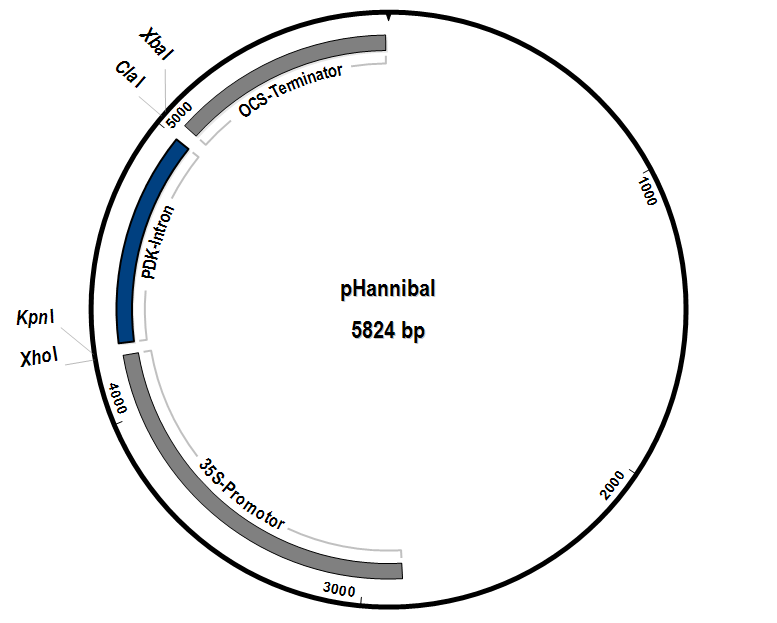
\includegraphics[scale=.3]{MaterialMethoden/Abb/pHannibalgb1}
\end{center}
\captionof{figure}[Plasmid pHannibal]{Plasmid pHannibal für den Aufbau von hpRNA-Konstrukten\\ \footnotesize blablabla}
\par


\section{Molekularbiologische Methoden}
\subsection{RNA-Präparation}
GitTest blablalbla bliblabvliua